\documentclass[a4paper]{article}

\usepackage[T1]{fontenc}
\usepackage[italian]{babel}
\usepackage[latin1]{inputenc}
\usepackage{graphicx}
\usepackage{float}
\usepackage[margin=2 cm]{geometry}
\usepackage{multirow}
\usepackage{multicol}
\author{Alberto Bordin, Giulio Cappelli}
\title{Analizzatore di spettro}
\date{27-28 novembre 2017}

\begin{document}
	\maketitle
	
\begin{abstract}
	Misura della separazione in frequenza dei modi principali di un laser HeNe.
	
	Misura della finezza di un Fabri-Perot.
\end{abstract}

\section{To do}

\begin{multicols}{2}

\section{Teoria}

\subsection{Laser HeNe}

\subsection{Fabri-Perot}

\section{Apparato sperimentale}

\end{multicols}

\begin{multicols}{2}
	
\section{Modi del laser HeNe}
Analizziamo la separazione in frequenza dei modi del laser HeNe a nostra disposizione.

In Figura \ref{fig:due_ordini.png} vediamo un esempio del segnale letto dall'oscilloscopio e visualizzato al PC. In rosso vediamo i picchi di trasmittivit� della cavit� Fabry-Perot e in blu la rampa del generatore di funzioni. Per ogni acquisizione salviamo sia l'immagine visualizzata che il file di testo associato al segnale. In Figura 

\end{multicols}

\begin{figure}[H]
	\centering
	\includegraphics[width=1\textwidth]{due_ordini.png}
	\caption{Due ordini dell'analizzatore.}
	\label{fig:due_ordini.png}
\end{figure}

\begin{figure}[H]
	\centering
	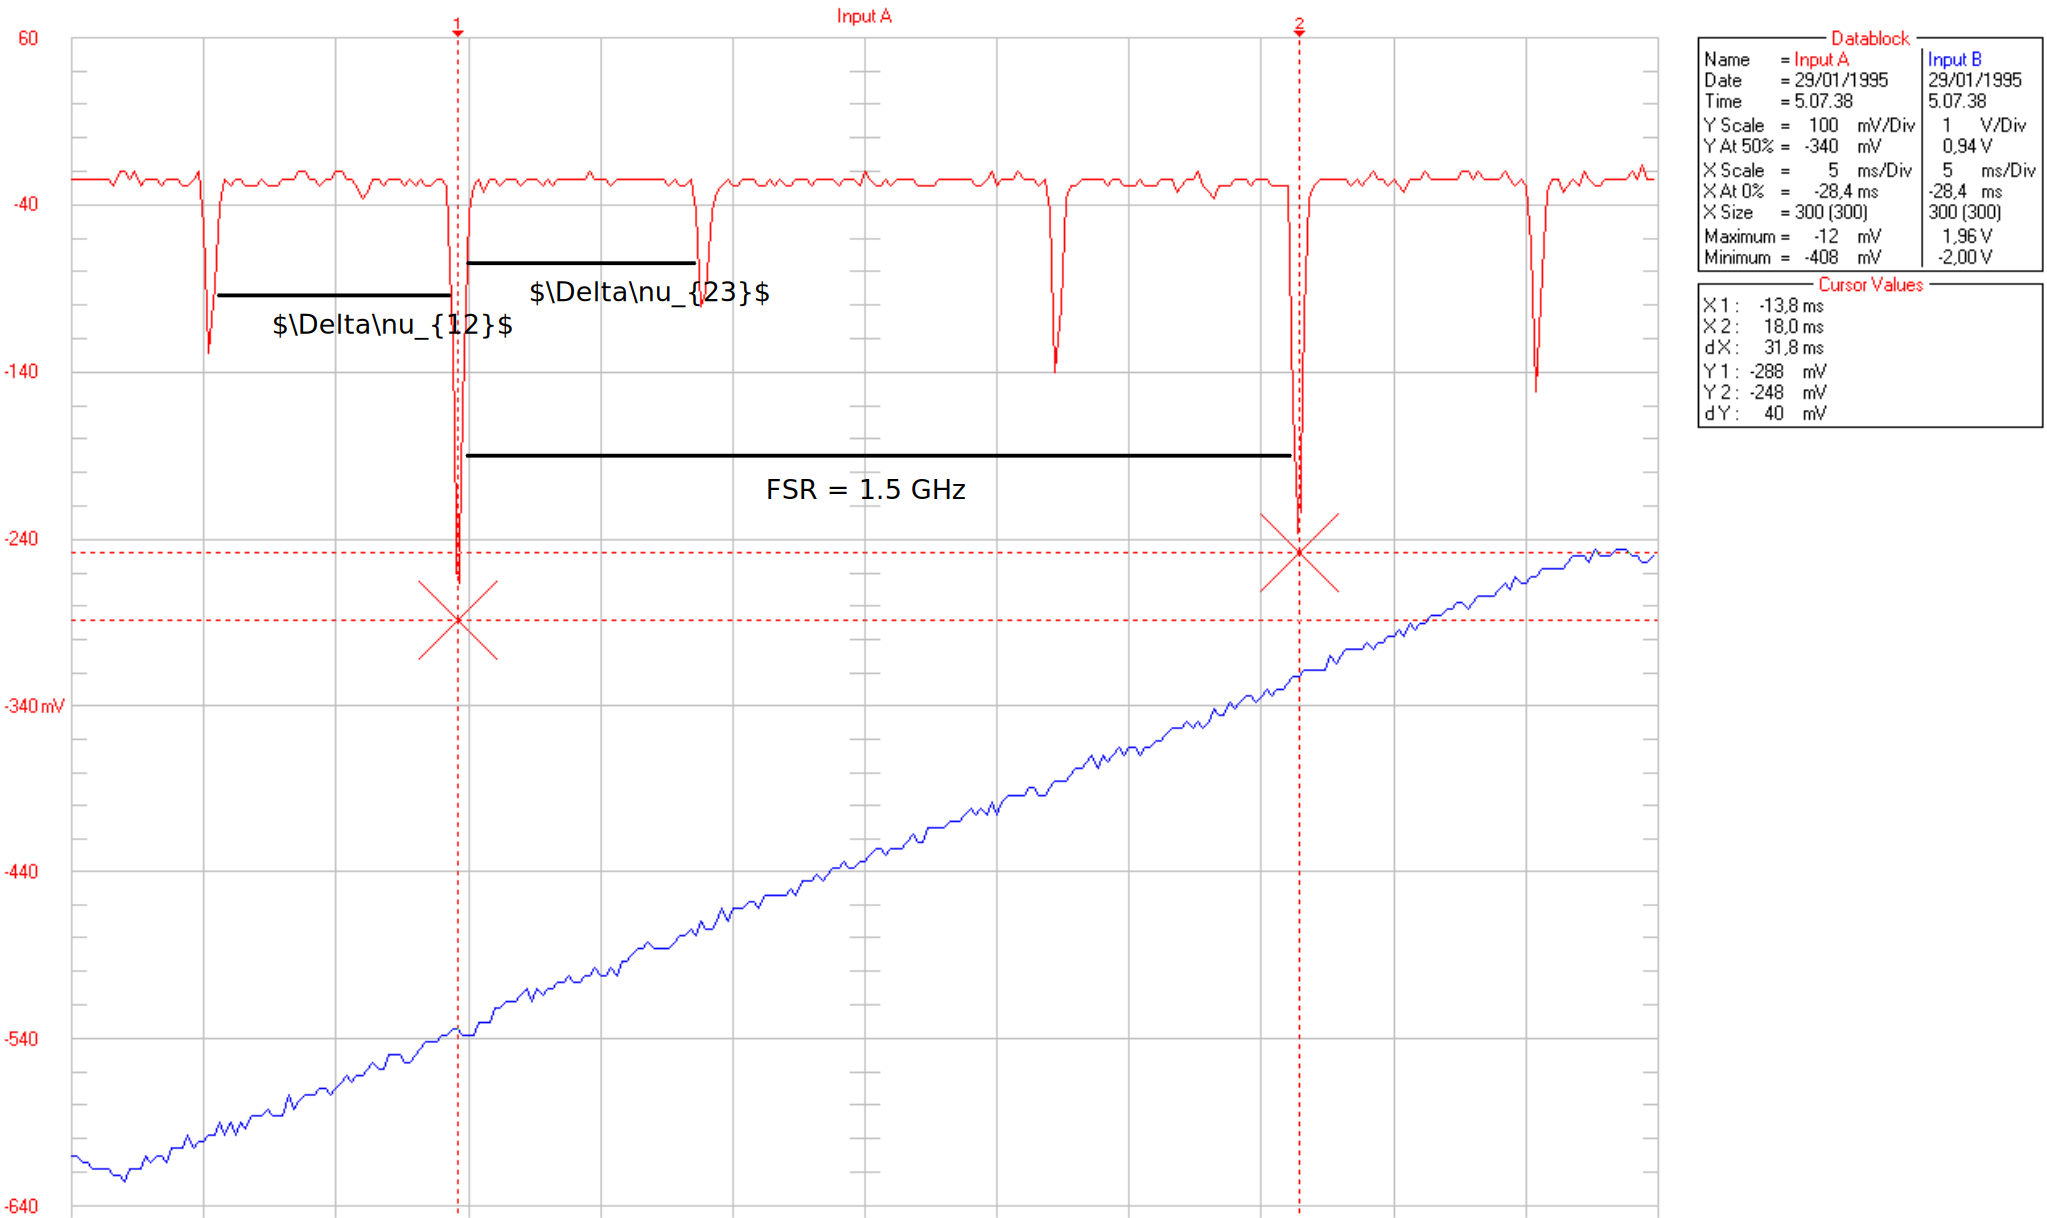
\includegraphics[width=1\textwidth]{un_ordine.png}
	\caption{Un ordine dell'analizzatore.}
	\label{fig:un_ordine.png}
\end{figure}

\begin{multicols}{2}
	
\subsection{Presa dati}



\end{multicols}

\begin{multicols}{2}
	
\section{Finezza del Fabri-Perot}

\end{multicols}
	
\end{document}

